% Prepared by Calvin Kent
%
% Assignment Template v19.02
%
%%% 20xx0x/MATHxxx/Crowdmark/Ax
%
\documentclass[12pt]{article} %
\usepackage{CKpreamble}
\usepackage{CKassignment}
\usepackage{tkz-euclide}
\usepackage{physics}
\usepackage{lmodern}
\usepackage{microtype}
\usepackage{tasks}
\usepackage{upgreek}
\usepackage{xcolor}
\usepackage{tikz}
\usetikzlibrary{angles,patterns,calc}
\usepackage{euscript}
\usepackage{tasks}
\usepackage{upgreek}
\usepackage[misc]{ifsym}


\usepackage{pgfplots}
\usepgfplotslibrary{polar}
\usepgflibrary{shapes.geometric}
\usetikzlibrary{calc}


\usepackage{euscript}
\usepackage{microtype}
\usepackage{upgreek}
\usepackage[misc]{ifsym}

%%Title
\title{Functions Final Exam - SOLUTIONS}
\date{February 3, 2021}

%%% Maths and science packages

\usepackage{amsmath,amsthm,amssymb}
\usepackage{pgfplots}
	\usetikzlibrary{
		calc,
		patterns,
		positioning
	}
	\pgfplotsset{
		compat=1.16,
		samples=200,
		clip=false,
		my axis style/.style={
			axis x line=middle,
			axis y line=middle,
			legend pos=outer north east,
			axis line style={
				->,
			},
			legend style={
				font=\footnotesize
			},
			label style={
				font=\footnotesize
			},
			tick label style={
				font=\footnotesize
			},
			xlabel style={
				at={
					(ticklabel* cs:1)
				},
				anchor=west,
				font=\footnotesize,
			},
			ylabel style={
				at={
					(ticklabel* cs:1)
				},
				anchor=west,
				font=\footnotesize,
			},
			xlabel= $x$,
			ylabel=$\vec d (\m \tx{[East]})$
		},
	}
	\tikzset{
		>=stealth
	}

\pgfplotsset{my style/.append style={axis x line=middle, axis y line=
middle, xlabel={}, ylabel={}, axis equal }}


%%% Tables and figures packages

\usepackage{float}
\usepackage{caption}
	\captionsetup{
		format=plain,
		labelfont=bf,
		font=small,
		justification=centering
	}

\newcounter{step}[section]
\newenvironment{step}[1][]
{\refstepcounter{step} \textbf{\\Step #1.}}

%%% Numbers and sets

\newcommand{\E}{\mathrm{e}}

\newcommand{\tx}[1]{\text{#1}}

\begin{document}
    \pagenumbering{arabic}
    % Start of class settings ...
    \renewcommand*{\coursecode}{MCR3U Quiz} % Quiz Title
    \renewcommand*{\assgnnumber}{1} % Quiz number
    \renewcommand*{\submdate}{November, 2021} % renew the date
    \renewcommand*{\studentfname}{\textbf{Name:}} % Student first name
    \renewcommand*{\studentlname}{} % Student last name
    %\renewcommand*{\studentnum}{SNumber} % Student number

    \renewcommand\qedsymbol{$\blacksquare$}
    \setfigpath
    % End of class settings 
    \newgeometry{left=18mm, right=18mm, top=22mm, bottom=22mm} % page is set to default values
    \fancyhfoffset[L,O]{0pt} % header orientation fixed
    % End of class settings
    %%% Note to user:
    % CTRL + F <CHANGE ME:> (without the angular brackets) in CKpreamble to specify graphics paths accordingly.
    % The command \circled[]{} accepts one optional and one mandatory argument.
    % Optional argument is for the size of the circle and mandatory argument is for its contents.
    % \circled{A} produces circled A, with size drawn for letter A. \circled[TT]{A} produces circled A with size drawn for TT.
    % https://github.com/CalvinKent/My-LaTeX
    %%%
    % Crowdmark assignment start


    %%%%%%%%%%%%%%%%%%%%%%%%%%%%%%%%%%%%%%%%%%%%%%%%%%%%%%%%%%%%%%%%%%%%%%%%%%%%%%%%%%%%%%%%%%%%%%%%%%%%%%%%
    %%%%%%%%%%%%%%%%%                  PROBLEM IDEAS                  %%%%%%%%%%%%%%%%%%%%%%%%%%%%%%%%%%%%%%
    %%%%%                   ----------------------------------------                                %%%%%%%%

    % --> Do a hard tangent line problem

	\maketitle
	\section{Preamble}
	This final exam covers everything we have learned in this course, with emphasize towards material after test 2. 
  Student's \emph{\textbf{must show all work}} to receive full marks.
	\section{Allowed Aids}
	The following aids are allowed on the Test
	\begin{itemize}
		\item Pencil, Pen, Eraser, Highlighter, Ruler, Protractor, Spare sheets of \textbf{blank} paper.
		\item Reference sheet \textbf{(Double sided paper preprepared by student)}
	\end{itemize}
	\section{Restrictions:}
  \begin{itemize}
		\item \textbf{NO} calculator's.
  \end{itemize}
	\section{Name and Date:}

  \vspace*{0.1cm}

	\begin{center}
	\noindent\begin{tabular}{ll}
		\makebox[3in]{\hrulefill} & \makebox[3in]{\hrulefill}\\
		Name & Date\\[8ex]% adds space between the two sets of signatures
	\end{tabular}
	\end{center}
	\newpage


\section*{Part A - Multiple Choice}
\begin{qstn} % qnumber, qname, qpoints
  Answer the following True/False questions,
  \begin{enumerate}
    \item Let $\mathcal{S} = \{1,2,3\}$, then $\mathcal{S} + \mathcal{S} = \mathcal{S} + \mathcal{S} +
      \mathcal{S}$.\\ 
       \textbf{\emph{Answer}}:\,\, \framebox[0.5in]{\textbf{True}} \,\,\,\,\,\, \textbf{False}\, , \,
       $\mathcal{S} + \mathcal{S} = \mathcal{S}$ and $\mathcal{S} + \mathcal{S} + \mathcal{S} = \mathcal{S}$.

    \item $\left(\sqrt{4} + \sqrt{64} \right) \not \in \mathbb N$.\\
       \textbf{\emph{Answer}}:\,\, \textbf{True} \,\,\,\,\,\, \framebox[0.5in]{\textbf{False}}\, , \,
       Note that $\sqrt{4}  + \sqrt{64} = 2 + 8 = 10$ and $10 \in \mathbb N$.

    \item The number $29$ is a prime number.\\
       \textbf{\emph{Answer}}:\,\, \framebox[0.5in]{\textbf{True}} \,\,\,\,\,\, \textbf{False}

    \item Let $T = \{x \in \Z \mid \left|x\right| = -1\} $, then $T$ is \textbf{not} empty.\\
       \textbf{\emph{Answer}}:\,\, \textbf{True} \,\,\,\,\,\, \framebox[0.5in]{\textbf{False}}\, , \,
       The absolute value of any number is always a positive number by definition, hence this set is empty.

    \item The vertex of 
      \[
        g(x) = 3\left( x + \sqrt{4}  \right)^2 - 4^2  
      \] is $(-4,-4)$.\\ 
       \textbf{\emph{Answer}}:\,\, \textbf{True} \,\,\,\,\,\, \framebox[0.5in]{\textbf{False}}\, , \,
       The vertex here is $(-2,-16)$.

    \item The vertex of,
      \[
            H(x) = -\left( x + 2 \right)^2 + 1
      .\] represents a minimum.\\
       \textbf{\emph{Answer}}:\,\, \textbf{True} \,\,\,\,\,\, \framebox[0.5in]{\textbf{False}}\, , \,
       The vertex here represents a maximum.


    \item Let $f(x) = \sqrt{x}$. Suppose we apply the following transformations to $f$,
      \begin{itemize}
        \item Reflection across the x-axis.
        \item Vertical stretch by a factor of $2$. 
        \item Horizontal compression by a factor of $2$.
        \item Horizontal shift, right by $2$ units.
        \item Vertical shift, down by $4$ units.
      \end{itemize}
      Then the corresponding transformation equation is $h(x) = -2f(2x - 4) - 4$.\\
       \textbf{\emph{Answer}}:\,\, \framebox[0.5in]{\textbf{True}} \,\,\,\,\,\, \textbf{False}

    \item Let $f(x) = \left|x\right|$, and let $h(x) = -f(2x + 4) - 5$ be a transformation of $f(x)$, then the
      corresponding coordinate transformation of $f$ is,
       \[
           \left( x,f(x) \right)  \longrightarrow \left( \frac{x + 4}{2}, -f(x) - 5 \right) 
      .\] 
       \textbf{\emph{Answer}}:\,\, \textbf{True} \,\,\,\,\,\, \framebox[0.5in]{\textbf{False}}\, , \,
        The correct coordinate transformation is $\left( \frac{x - 4}{2}, -f(x) - 5 \right)$.

    \item Let $f \colon \R \to \R$, $f(x) = 2\sqrt{x} + 1$ be a function. Then $f$ is not invertible. \\
      \textbf{Hint: }Try using the Horizontal line test.\\
       \textbf{\emph{Answer}}:\,\, \textbf{True} \,\,\,\,\,\, \framebox[0.5in]{\textbf{False}}\, , \,
       Try using the horizontal line test to see why.

      \newpage

    \item Let $ \mathcal{X} = \{45^{\circ}, 60^{\circ}, 240^{\circ}\} $ and 
      $ \mathcal{Y} = \left\{0,1,\sqrt{3} \right\} $ be sets, define the
            following function, 
            \begin{itemize}
              \item $\mathcal{\omega} \colon \mathcal{X} \to \mathcal{Y}$.
              \item $\mathcal{\omega}(x) = \tan(x)$.
            \end{itemize}
            Then $\omega$ is an invertible function.\\
       \textbf{\emph{Answer}}:\,\, \textbf{True} \,\,\,\,\,\, \framebox[0.5in]{\textbf{False}}\, , \,
       Note that $\tan (60^{\circ}) = \tan (240^{\circ}) = \sqrt{3}$ and hence $\omega$ fails to be injective which
       asserts that it fails to be invertible as well.

    \item Let $\triangle PQR$ be a \textbf{right triangle} with angle $\angle PQR = 60^{\circ}$ and 
        \textit{hypotenuse} $PQ = 8$. Then $QR = 4$.\\
       \textbf{\emph{Answer}}:\,\, \framebox[0.5in]{\textbf{True}} \,\,\,\,\,\, \textbf{False}

    \item The exact value of 
      \[ 
        \sin 150^{\circ} \cdot \sec 240^{\circ} + \tan 240^{\circ}\tan 30^{\circ} = 0
      \]
       \textbf{\emph{Answer}}:\,\, \framebox[0.5in]{\textbf{True}} \,\,\,\,\,\, \textbf{False}

    \item Let $\triangle PQR$ be a \textbf{right triangle} with $PQ = 6$ and $QR = 3\sqrt{3}$. Then, $\angle PQR = 60^{\circ}$.
      \begin{center}
          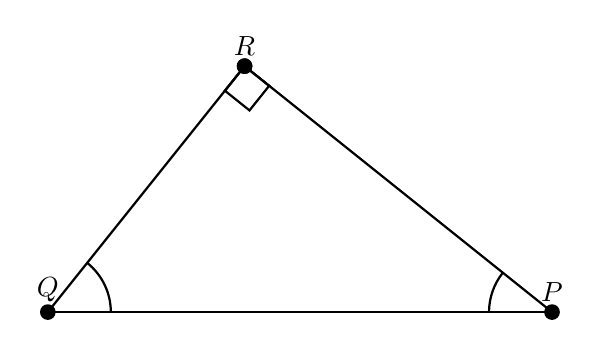
\begin{tikzpicture}[thick]
          \coordinate (Q) at (0,2);
          \coordinate (R) at (2.49878019,5.123475);
          \coordinate (P) at (6.403124,2);

          \draw[black] (0,2) -- (6.403124,2) node[circle,fill,inner sep=2pt]{} node[above]{$P$};
          \draw[black] (0,2) -- (2.49878019,5.123475) node[circle,black,fill,inner sep=2pt]{} node[above]{$R$};
          \draw[black] (6.403124,2) -- (2.49878019,5.123475) node[circle,black,fill,inner sep=2pt]{};
          \draw[black] (0,2) node[circle,black,fill,inner sep=2pt]{} node[above]{$Q$};

          \tkzMarkRightAngle[size=0.4,opacity=1](Q,R,P)% square angle here

          \tkzMarkAngle[fill= orange,size=0.8cm,%
          opacity=1](P,Q,R)
          \tkzLabelAngle[pos = 1.2](P,Q,R){}

          \tkzMarkAngle[fill= orange,size=0.8cm,%
          opacity=1](R,P,Q)
          \tkzLabelAngle[pos = 1.2](R,P,Q){}


          \end{tikzpicture}
      \end{center}
       \textbf{\emph{Answer}}:\,\, \textbf{True} \,\,\,\,\,\, \framebox[0.5in]{\textbf{False}}\, , \,
       $\angle PQR = 30^{\circ}$.

    \item $\sin 330^{\circ} = -0.5$.\\
       \textbf{\emph{Answer}}:\,\, \framebox[0.5in]{\textbf{True}} \,\,\,\,\,\, \textbf{False}

    \item Suppose we have the standard coordinates $\vb P\left( 2 , -\sqrt{12}\right) $, then the corresponding polar coordinates
        are $\vb P(4,60^{\circ})$.\\
       \textbf{\emph{Answer}}:\,\, \textbf{True} \,\,\,\,\,\, \framebox[0.5in]{\textbf{False}}\, , \,
       The corresponding polar coordinates are $\vb P(4, 300^{\circ})$.

    \item $\sqrt{4^{4}\cdot 3^{2}\cdot 2} = 48\sqrt{2}$. \\
       \textbf{\emph{Answer}}:\,\, \framebox[0.5in]{\textbf{True}} \,\,\,\,\,\, \textbf{False}

  \end{enumerate}
\end{qstn}

\newpage

\section*{Part B}
\begin{qstn}
  Explain in your own words, what is a function?
  \begin{solution}
    Suppose we have two sets $\mathcal{S}, \mathcal{T}$, a function from the set $\mathcal{S}$ to $\mathcal{T}$,
    is a rule which assigns to each element in $\mathcal{S}$ a corresponding element in $\mathcal{T}$.
  \end{solution}
\end{qstn}

\vspace*{2cm}

\begin{qstn}
  Given a function $f \colon A \to B$, explain in your own words, what is the definition of the range of $f$, 
  $\mathcal{R}_f$, what does it contain? Is it necessarily true that $\mathcal{R}_f = B$?
  \begin{solution}
    The range $\mathcal{R}_f$ is a \emph{set} which contains all of the output values of the function after
    processing each element from the domain. It is \emph{not} necessarily true that $\mathcal{R}_f = B$ but rather
    this a special case of surjectiveness.
  \end{solution}
\end{qstn}

\vspace*{2cm}

\begin{qstn}
  Given a function $f \colon A \to B$, explain in your own words what do we mean when we say that $f$ is
  invertible?
  \begin{solution}
    We say that $f$ is invertible if it is both surjective and injective. By surjective, we mean that each element
    in the co-domain $B$ is mapped to and by injective we mean that no two elements in the domain $A$ map to the
    same element in the co-domain $B$.
  \end{solution}
\end{qstn}

\vspace*{2cm}

\begin{qstn}
  Explain what the horizontal line test is as well as the vertical line test.
  \begin{solution}
    For a function $f$, the horizontal line test is used to provide a certificate of invertibility while the
    vertical line test asserts wether or not $f$ is a proper function.
  \end{solution}
\end{qstn}

\newpage

\section*{Part C}

\begin{qstn}
  Let $F(x) = x^3  + 1$, and $G(x) = 2x^2 + x - 1$ be functions,
  \begin{enumerate}[label=(\alph*)]
    \item Compute $F(-1)$.
      \begin{solution}
        \[
              F(-1) = (-1)^{3} + 1 = -1 + 1 = 0
        .\] 
      \end{solution}
      \vspace*{1cm}

    \item Compute  $G(2)$. 
      \begin{solution}
        \[
              G(2) = 2(2)^2 + 2 - 1 = 8 + 2 - 1 = 9
        .\] 
      \end{solution}
      \vspace*{1cm}

    \item Compute $F(G(1))$. 
      \begin{solution}
        \begin{align*}
          G(1) &= 2(1)^2 + 1 - 1 = 2 + 1 - 1 = 2\\
          F(G(1)) &= F(2) = (2)^3 + 1 = 8 + 1 = 9
        .\end{align*}
      \end{solution}
      \vspace*{1cm}

    \item Compute $G(F(F(0)))$.
      \begin{solution}
        \begin{align*}
          F(0) &= (0)^3 + 1 = 1\\
          F(F(0)) &= F(1) = (1)^3 + 1 = 1 + 1 = 2\\
          G(F(F(0))) &= G(2) = 9
        .\end{align*}
      \end{solution}
  \end{enumerate}
\end{qstn}

\newpage

\begin{qstn}
  Let $g(x) = 2x^2 - 4x + 4$,
  \begin{enumerate}[label=(\alph*)]
    \item How many solutions will $g(x)$ have?
      \begin{solution}
        Using the discriminant formula,
        \begin{align*}
          d &= b^2 - 4ac\\
            &= (4)^2 - 4(2)(4)\\
            &= 16 - 32\\
            &= -16
        .\end{align*}
        Since $d < 0$,  $g(x)$ will have \emph{no} solutions.
      \end{solution}

        \vspace*{1cm}

    \item Convert $g(x)$ into vertex form by completing the square.
      \begin{solution}
        \begin{step}[1]
          \begin{align*}
            0 &= b^2 - 4at\\
            0 &= (-4)^2 - 4(2)t\\
            0 &= 16 - 8t\\
            t &= 2
          .\end{align*}
        \end{step}

        \begin{step}[2]
          Since $a \cdot b = 2 \cdot -4 = -8$, we conclude that $a \cdot b < 0$, hence,
          \begin{align*}
            g(x) &= a\left( x - \sqrt{\frac{t}{a}}  \right) ^2 + [c - t]\\
                 &= 2\left( x - \sqrt{\frac{2}{2}} \right) ^2 + [4 - 2]\\
                 &= 2\left( x - 1 \right) ^2 + 2
          .\end{align*}
        \end{step}
      \end{solution}

        \vspace*{1cm}

    \item Does the vertex of $g(x)$ represent a minimum or maximum, justify your answer.
      \begin{solution}
        Since $a = 2$ and $2 > 0$, the vertex of $g(x)$ represents a \emph{minimum}.
      \end{solution}

  \end{enumerate}
\end{qstn}

\newpage

\begin{qstn}
  Determine the inverse function for the following functions,
  \begin{enumerate}[label=(\alph*)]
    \item $F(x) = -8x + 16$.
      \begin{solution}
        Proceeding with the inverse algorithm,
        \begin{align*}
          F(x) &= -8x + 16\\
          y &= -8x + 16\\
          y - 16 &= -8x\\
          x &= -\frac{1}{8}\left( y - 16 \right)\\
          F^{-1}(x) &= -\frac{1}{8}\left( x - 16 \right)
        .\end{align*}
      \end{solution}

        \vspace*{1cm}

    \item $G(x) = 2\sqrt{x + 8} - 4$.
      \begin{solution}
        \begin{align*}
          G(x) &= 2\sqrt{x + 8}  - 4\\
          y &= 2\sqrt{x + 8}  - 4\\
          y + 4 &= 2\sqrt{x + 8}\\
          \frac{y + 4}{2} &= \sqrt{x + 8}\\
          \left( \frac{y + 4}{2} \right) ^2 &= x + 8\\
          x &= \left( \frac{y + 4}{2} \right) ^2 - 8\\
          G^{-1}(x) &= \left( \frac{x + 4}{2} \right) ^2 - 8
        .\end{align*}
      \end{solution}
  \end{enumerate}
\end{qstn}

\newpage
\begin{qstn}
Simplify the following exponential expression, \textbf{leave your answer with positive exponents}.
\[
   \frac{\left(2x^2x^4y^{-3}z^{-4} \right)^{2}}{\left(8x^{-2}y^{-5}z^{2} \right)^{2}}
\] 

  \begin{solution}
    \begin{align*}
          \frac{\left(2x^2x^4y^{-3}z^{-4} \right)^{2}}{\left(8x^{-2}y^{-5}z^{2} \right)^{2}} 
          &= \frac{2^{2}x^{12}y^{-6}z^{-8} }{8^{2}x^{-4}y^{-10}z^{4} }\\
          &= \frac{4x^{16}y^{10}}{64y^{6}z^{12}}\\
          &= \frac{4x^{16}y^{10-6}}{64z^{12}}\\
          &= \frac{x^{16}y^{4}}{16z^{12}}\\
    \end{align*}
  \end{solution}

\end{qstn}
        \vspace*{1.5cm}


\begin{qstn}
  Evaluate the following,
\[
      \left( 16^{\frac{4}{4}} \right) \left( 9^{\frac{3}{2}} \right) \left( 4^{\frac{1}{2}} \right) \left( 2^{-3}
      \right)
\] 

  \begin{solution}
    \begin{align*}
      \left( 16^{\frac{4}{4}} \right) \left( 9^{\frac{3}{2}} \right) \left( 4^{\frac{1}{2}} \right) \left( 2^{-3}
      \right)
      &= \frac{\left( 16^{1} \right) \left( 9^{\frac{1}{2}} \right) ^{3}\left( 4^{\frac{1}{2}} \right)}{2^{3}}\\
      &= \frac{16 \left( 3 \right) ^{3}2}{8}\\
      &= 2 \left( 3 \right) ^{3}2\\
      &= 4(27)\\
      &= 108
    \end{align*}
  \end{solution}
  
\end{qstn}

\newpage
\begin{qstn}
  Simply the following radical expressions.
  \begin{enumerate}[label=(\alph*)]
    \item \[
        2\sqrt{27} + 3\sqrt{3} - 2\sqrt{12} + \sqrt{48}  
    \] 
    \begin{solution}
      \begin{align*}
        2\sqrt{27} + 3\sqrt{3} - 2\sqrt{12} + \sqrt{48} 
        &= 2\sqrt{9 \cdot 3}  + 3\sqrt{3} - 2\sqrt{4 \cdot 3} + \sqrt{16 \cdot 3}\\
        &= 2\sqrt{9}\sqrt{3} + 3\sqrt{3} - 2\sqrt{4}\sqrt{3} + \sqrt{16}\sqrt{3}\\
        &= 2(3)\sqrt{3} + 3\sqrt{3} - 2(2)\sqrt{3}  + 4\sqrt{3}\\
        &= 6\sqrt{3} + 3\sqrt{3} - 4\sqrt{3} + 4\sqrt{3}\\
        &= 9\sqrt{3} 
      .\end{align*}
      
    \end{solution}


  \item \[
      \left( 2\sqrt{2} + \sqrt{3} \right) \left( 5\sqrt{3}  + 3\sqrt{2}\right)
  \] 
  \begin{solution}
    \begin{align*}
      \left( 2\sqrt{2} + \sqrt{3} \right) \left( 5\sqrt{3}  + 3\sqrt{2}\right)
      &= \left( 2\sqrt{2}\right) \left( 5\sqrt{3}\right) + \left( 2\sqrt{2}\right) \left( 3\sqrt{2}\right) 
              + \left( \sqrt{3}\right) \left( 5\sqrt{3}\right) + \left( \sqrt{3}\right)\left( 3\sqrt{2}\right)\\
      &= 10\sqrt{2}\sqrt{3} + 6\sqrt{2}\sqrt{2} + 5\sqrt{3}\sqrt{3} + 3\sqrt{3}\sqrt{2}\\
      &= 10\sqrt{2\cdot 3} + 6\sqrt{2\cdot 2} + 5\sqrt{3\cdot 3} + 3\sqrt{3\cdot 2}\\
      &= 10\sqrt{6}  + 6\sqrt{4} + 5\sqrt{9} + 3\sqrt{6}\\
      &= 13\sqrt{6} + 6(2) + 5(3)\\
      &= 12 + 15 + 13\sqrt{6} \\
      &= 27 + 13\sqrt{6} 
    \end{align*}
  \end{solution}
  \end{enumerate}
\end{qstn}

\newpage

\begin{qstn}
  Simplify the following,
  \begin{enumerate}[label=(\alph*)]
    \item \[
        \frac{2x^2 - 8x}{x^2 - 11x + 18} \times \frac{2x^{2} - 7x + 6}{x^2 - 5x + 4}
    \] 

    \begin{solution}
      \begin{align*}
        \frac{2x^2 - 8x}{x^2 - 11x + 18} \times \frac{2x^{2} - 7x + 6}{x^2 - 5x + 4}
        &= \frac{2x(x - 4)}{(x-9)(x-2)} \times \frac{(2x - 3)(x - 2)}{(x-4)(x-1)}\\
        &= \frac{2x(x - 4)(2x - 3)(x - 2)}{(x-9)(x-2)(x-4)(x-1)}\\
        &= \frac{2x\cancel{(x - 4)}(2x - 3)\cancel{(x - 2)}}{(x-9)\cancel{(x-2)}\cancel{(x-4)}(x-1)}\\
        &= \frac{2x(2x - 3)}{(x-9)(x-1)}
      .\end{align*}
      
    \end{solution}

    \newpage

  \item \[
      \frac{x}{x^2 - 5x + 6} - \frac{3}{x^2 - 4x + 4}
  \] 
  \begin{solution}
    Let $A(x) = x$,  $B(x) = x^2 - 5x + 6$, $C(x) = 3$,  $D(x) = x^2 - 4x + 4$.
    \begin{align*}
      \frac{x}{x^2 - 5x + 6} - \frac{3}{x^2 - 4x + 4}
      &= \frac{x}{(x-3)(x-2)} - \frac{3}{(x-2)(x-2)}
    \end{align*}
    Notice that the LCD here is,
    \begin{align*}
      L(x) &= \frac{B(x)\cdot D(x)}{\gcd \left( B(x),D(x) \right) }\\
            &= \frac{(x-3)(x-2)\cdot (x-2)(x-2)}{\gcd \left((x-3)(x-2), (x-2)(x-2) \right) }\\
            &= \frac{(x-3)(x-2) (x-2)(x-2)}{(x-2)}\\
            &= \frac{(x-3)(x-2) \cancel{(x-2)}(x-2)}{\cancel{(x-2)}}\\
            &=(x-3)(x-2)(x-2)
    \end{align*}
    The missing factor for $B(x)$ is  $R(x) = (x-2)$ and the missing factor for  $D(x)$ is  $Q(x) = (x - 3)$, and
    hence,
    \begin{align*}
      \frac{x}{x^2 - 5x + 6} - \frac{3}{x^2 - 4x + 4}
      &= \frac{x}{(x-3)(x-2)} - \frac{3}{(x-2)(x-2)}\\
      &= \frac{x(x-2) - 3(x-3)}{(x-3)(x-2)(x-2)}\\
      &= \frac{x^2 - 2x - 3x^2 + 9}{(x-3)(x-2)(x-2)}\\
      &= \frac{-2x^2 - 2x + 9}{(x-3)(x-2)(x-2)}
    \end{align*}
  \end{solution}
  \end{enumerate}

\end{qstn}

\newpage

\begin{qstn}
 For each of the following, you are given a trigonometric ratio, solve for $\theta$. 
  Assume that each angle  $\theta$ lies in the \textbf{fourth} quadrant.
  \textbf{(You can use the circle below if it helps)}.
  \begin{enumerate}[label=(\alph*)]
    \item \[
      \cos \theta_1 = \frac{1}{2}
    .\] 
    \begin{solution}\texttt{  }
      \begin{step}[1]
         \begin{center}
          \begin{tikzpicture}
            \begin{axis}[
                my style,
                ytick=\empty,
                xtick=\empty,
                xticklabels=\empty,
                width=0.7\textwidth,
                height=0.55\textwidth,
                yticklabels=\empty,
              ]

              \draw (axis cs: 0, 0) circle [radius=20];% I've set the radius to 10 only for better show the image
              \draw[->] (10,0) arc (0:300:10) node[midway]{};
              \draw (0,0) -- (300:20) node[midway, above] {};
              \draw (300:20) node[circle,fill,draw,inner sep=2pt] {};

              \draw[-] (6,0) arc (0:-60:6) node[midway]{};

              \node[label={135:{\textcolor{black}{$\theta_1$}}},circle,inner sep=0.5pt] at (10,8) {};
              \node[label={135:{\textcolor{black}{$\alpha$}}},circle,inner sep=0.5pt] at (8,-4) {};

              \addplot[domain=-21:21, white]{-x};

            \end{axis}
          \end{tikzpicture}
         \end{center}
      \end{step}

      \begin{step}[2]
        \[
            \alpha = \cos^{-1}\left( \left|\frac{1}{2}\right| \right) = \cos^{-1}\left( \frac{1}{2} \right)
                      = 60^{\circ}
        .\] 
      \end{step}

      \begin{step}[3]
        \[
            \theta_1 = 360^{\circ} - \alpha = 360^{\circ} - 60^{\circ} = 300^{\circ}
        .\] 
      \end{step}
   \end{solution}
      
   \newpage

    \item \[
      \tan \theta_2 = -\frac{1}{\sqrt{3}} 
    .\] 
    \begin{solution}\texttt{  }
      \begin{step}[1]
         \begin{center}
          \begin{tikzpicture}
            \begin{axis}[
                my style,
                ytick=\empty,
                xtick=\empty,
                xticklabels=\empty,
                width=0.7\textwidth,
                height=0.55\textwidth,
                yticklabels=\empty,
              ]

              \draw (axis cs: 0, 0) circle [radius=20];% I've set the radius to 10 only for better show the image
              \draw[->] (10,0) arc (0:330:10) node[midway]{};
              \draw (0,0) -- (330:20) node[midway, above] {};
              \draw (330:20) node[circle,fill,draw,inner sep=2pt] {};

              \draw[-] (6,0) arc (0:-30:6) node[midway]{};

              \node[label={135:{\textcolor{black}{$\theta_2$}}},circle,inner sep=0.5pt] at (10,8) {};
              \node[label={135:{\textcolor{black}{$\alpha$}}},circle,inner sep=0.5pt] at (8.5,-3) {};

              \addplot[domain=-21:21, white]{-x};

            \end{axis}
          \end{tikzpicture}
         \end{center}
      \end{step}

      \begin{step}[2]
        \[
            \alpha = \tan^{-1}\left( \left|-\frac{1}{\sqrt{3}}\right| \right) = \tan^{-1}\left(\frac{1}{\sqrt{3}}\right)
                      = 30^{\circ}
        .\] 
      \end{step}

      \begin{step}[3]
        \[
            \theta_1 = 360^{\circ} - \alpha = 360^{\circ} - 30^{\circ} = 330^{\circ}
        .\] 
      \end{step}
   \end{solution}

  \end{enumerate}
\end{qstn}

\newpage

\section*{Part D - Solve one of the two problems}

\begin{qstn}
  Suppose we have two standard coordinates $\vb P(x_1,y_1)$ and $\vb Q(x_2,y_2)$. Recall that the distance between
  these two points is given by the following formula,
  \[
        \operatorname{dist} = \sqrt{\left( x_2 - x_1 \right) ^2 + \left( y_2 - y_1 \right) ^2} 
  .\] 

  Given polar coordinates $\vb R(2,150^{\circ})$ and $ \vb T(2,330^{\circ})$, compute the distance between them.
  \begin{solution}
    The strategy here is to convert each coordinate to standard coordinates and to use the distance formula from
    there,
    \begin{step}[1]
      Convert $\vb R(2,150^{\circ})$ to standard coordinates.
      \begin{multicols}{2}
            \begin{align*}
              x &=   r\cos \theta\\
                &= 2 \cos 150^{\circ}\\
                &= 2(\pm \cos \alpha)\\
                &= 2(- \cos 30^{\circ})\\
                &= 2\left( -\frac{\sqrt{3}}{2}\right) \\
                &= -\sqrt{3}
              \end{align*}

        \columnbreak
              \begin{align*}
              y &=   r\sin \theta\\
                &= 2\sin 150^{\circ}\\
                &= 2(\pm \sin \alpha)\\
                &= 2(\sin 30^{\circ})\\
                &= 2\left( \frac{1}{2} \right) \\
                &= 1
             \end{align*}
        
      \end{multicols}
      Hence $\vb R\left( -\sqrt{3}, 1\right)$.
    \end{step}

    \begin{step}[2]
      Convert $\vb T(2,330^{\circ})$ to standard coordinates.
      \begin{multicols}{2}
            \begin{align*}
              x &=   r\cos \theta\\
                &= 2 \cos 330^{\circ}\\
                &= 2(\pm \cos \alpha)\\
                &= 2(\cos 30^{\circ})\\
                &= 2\left( \frac{\sqrt{3}}{2}\right) \\
                &= \sqrt{3}
              \end{align*}

        \columnbreak
              \begin{align*}
              y &=   r\sin \theta\\
                &= 2\sin 330^{\circ}\\
                &= 2(\pm \sin \alpha)\\
                &= 2(- \sin 30^{\circ})\\
                &= 2\left(- \frac{1}{2} \right) \\
                &= -1
             \end{align*}
        
      \end{multicols}
      Hence $\vb T\left( \sqrt{3}, -1\right)$.
    \end{step}

    \newpage

    \begin{step}[3]
      Using the distance formula,
      \begin{align*}
        \operatorname{dist} &= \sqrt{\left( x_2 - x_1 \right) ^2 + \left( y_2 - y_1 \right) ^2} \\
                            &= \sqrt{\left( \sqrt{3} - \left( -\sqrt{3}\right)   \right) ^2 +
                                    \left( -1 - 1\right) ^2} \\
                            &= \sqrt{\left( 2\sqrt{3}\right) ^2 +
                                    \left( -2\right) ^2} \\
                            &= \sqrt{\left( 2\right)^2\left( \sqrt{3}\right)^2 +
                                    \left( -2\right) ^2} \\
                            &= \sqrt{4(3) + 4} \\
                            &= \sqrt{16} \\
                            &= 4
      .\end{align*}
    \end{step}
    Hence the distance between the two points is dist $= 4$.
  \end{solution}
\end{qstn}

\vspace*{1cm}

\begin{qstn}
The figure below is composed of a kite and a circle. The radius of the circle is $4$ and the point $M$
represents the midpoint of the circle. $\angle ADM = 30^{\circ}$ and $MC = 20$. If the area of the circle is $A_c =
48$, then determine the area of the
shaded region \emph{in exact form}.\\ (\textbf{Hint:} A kite has unqiue symmetric relationships which assert that
$\angle ADM = \angle ABM$,  $\angle MDC = \angle MBC$, $DM = MB$,  $AD = AB$,  $BC = DC$).
        \begin{center}
          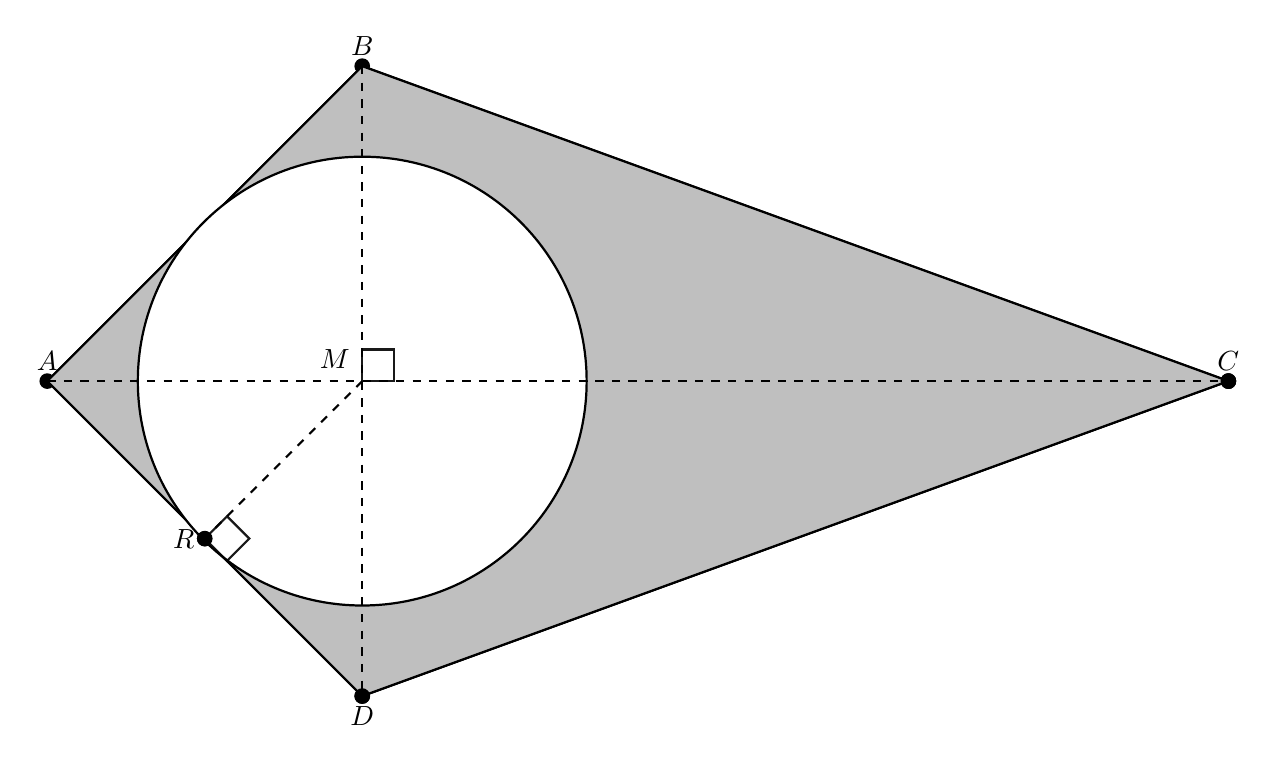
\begin{tikzpicture}[thick]
          \coordinate (A) at (0,0);
          \coordinate (B) at (4,4);
          \coordinate (D) at (4,-4);
          \coordinate (M1) at (2,-2);
          \coordinate (C) at (15,0);
          \coordinate (M) at (4,0);



          \draw[black] (A) -- (B) node[circle,black,fill,inner sep=2pt]{} node[above]{$B$};
          \draw[black] (A) -- (D) node[circle,black,fill,inner sep=2pt]{} node[below]{$D$};
          \draw[black] (B) -- (C) node[circle,black,fill,inner sep=2pt]{} node[above]{$C$};;
          \draw[black] (D) -- (C) node[circle,black,fill,inner sep=2pt]{};
          \draw[black] (A) node[circle,black,fill,inner sep=2pt]{} node[above]{$A$};
          \draw[black] (M1) node[circle,black,fill,inner sep=2pt]{} node[left]{$R$};
          \draw[black] (M) node[circle,black,fill,inner sep=2pt]{};

          \draw[fill=gray!50]  (A) -- (B) -- (C) -- (D) -- cycle;

          \draw[fill=white] (4,0) circle [radius=2.85];% I've set the radius to 10 only for better show the image
          \draw[dashed] (B) -- (D) node[circle,black,fill,inner sep=2pt]{};
          \draw[dashed] (A) -- (C) node[circle,black,fill,inner sep=2pt]{};
          \draw[dashed] (M) -- (M1) node[circle,black,fill,inner sep=2pt]{};

          \tkzMarkRightAngle[size=0.4,opacity=0.9](B,M,C)% square angle here
          \tkzMarkRightAngle[size=0.4,opacity=0.9](M,M1,D)% square angle here

          \node[label={135:{\textcolor{black}{$M$}}},circle,inner sep=0.5pt] at (4,0) {};

          \end{tikzpicture}

      \end{center}

      \newpage
  
      \begin{solution}
        Since point $M$ corresponds to the midpoint of the circle and the radius of the circle is $4$, we conclude
        that $RM = 4$. If we analyse triangle  $MRD$, then we can use the fact that $\angle ADM = 30^{\circ}$ to
        conclude that $\angle RMD = 60^{\circ}$. We can solve for side $MD$ by,
        \begin{align*}
          \cos \angle RMD &= \frac{RM}{MD}\\
          \cos 60^{\circ} &= \frac{4}{MD}\\
          \frac{1}{2} &= \frac{4}{MD}\\
          MD &= 8
        .\end{align*}
        Notice that triangle $AMD$ is a right triangle at vertex  $M$, hence we can use a tangent ratio to solve
        for side  $AM$,
         \begin{align*}
           \tan \angle ADM &= \frac{AM}{MD}\\
           \tan 30^{\circ} &= \frac{AM}{8}\\
           \frac{1}{\sqrt{3}} &= \frac{AM}{8}\\
           AM &= \frac{8}{\sqrt{3}}
        .\end{align*}
        At this point we can solve for the area of triangle $ABD$, note that side  $BD = BM + MD = MD + MD = 8 + 8
        = 16$, where the last line of equality follows from the symmetric relations on kites. Hence,
         \[
            A_{\triangle ABD} = \frac{1}{2}\left( BD \cdot AM \right) = \frac{1}{2}\left( 16\cdot \frac{8}{\sqrt{3} } \right)
                               = \frac{64}{\sqrt{3}}
        .\] 
        We can also solve for the area of triangle $BDC$,
        \[
            A_{\triangle BDC} = \frac{1}{2}\left( BD \cdot MC \right)  = \frac{1}{2}\left( 16\cdot 20 \right) 
                              = 160
        .\] 
        Let the area of the shaded region be $A_S$, we obtain the area by first determining the area of the
        kite, we can do so by taking the sum of the two areas we have previously
        determined, and then subtracting the area of the circle from the result of the summation.
        \begin{align*}
          A_S &= A_{kite} - A_c\\
              &= A_{\triangle ABD} + A_{\triangle BDC} - A_c\\
              &= \frac{64}{\sqrt{3}} + 160 - 48\\
              &= \frac{64}{\sqrt{3}} + 112
        .\end{align*}
      \end{solution}
\end{qstn}



\end{document}






























